\section{Entity relationship diagram}
\subsection{préambule}
Dans cette partie, nous allons parler de la modélisation de la base de donnée. Chaque sous-section parlera d'une relation. Dans ces sous-sections, nous parlerons du fonctionnement de certains attributs et nous définirons nos clés primaires et étrangères.
\\ \\ 
De manière générale, nous avons fait en sorte d'obtenir le moins de rendondance possible entre les différentes relations pour convenir au mieux à la 3NF\footnote{ \url{https://en.wikipedia.org/wiki/Third_normal_form}}.
\subsection{utilisateur}
Nous partons du principe qu'un fournisseur et un client sont avant tout des utilisateurs de l'application. De ce fait, les deux personnes auront un identifiant "id"("u" + 9 digits). Cet identifiant représente la quantième personne qui a été inscrite. Par exemple, si je suis le premier utilisateur alors j'aurai l'identifiant : u000000000.
\\ \\
A noter que le mot de passe sera stocké dans la base de donné après avoir été hashé par l'algorithme bycrypt\footnote{\url{https://fr.wikipedia.org/wiki/Bcrypt}} pour éviter toute fuite dans le cas où la base de donnée serait compromise.
\\ \\
PK(utilisateur) = \texttt{id}
\\ \\
FK(utilisateur) REFS fournisseur = \texttt{id}
\\
FK(utilisateur) REFS client = \texttt{id}
\newpage
\subsection{langue}
Dans cette relation, nous posons que l'utilisateur peut avoir plusieurs langues. De ce fait, nous avons une clé primaire composé. 
\\ \\
De plus, la langue enregistrée peut être une langue préférée (1 si c'est le cas, 0 sinon). 
\\ \\
Ensuite, un attribut binaire \texttt{langue\_actuelle} est stocké. Cet attribut nous permet de savoir quel langue l'utilisateur est en train d'utiliser ou a utilisé pendant sa dernière session (1 si c'est le cas, 0 sinon). 
\\ \\
PK(langue) = \texttt{id} et \texttt{langue\_enregistrée}
\\ \\
FK(langue) REFS utilisateur = \texttt{id}
\subsection{client}
Du coté de la relation "client", nous y trouvons un seul attribut. Cela nous permet d'avoir un utilisateur ayant aucun portefeuille.
\\ \\
PK(client) = \texttt{id\_client}
\subsection{portefeuille}
L'adresse sera définit comme : nomdeville-nomderue-numérodemaison. 
\\ \\
PK(portefeuille) = \texttt{adresse}
\\ \\
FK(portefeuille) REFS client = \texttt{id\_client}
\subsection{contrat du portefeuille}
 Dans "contrat du portefeuille" et pour tout autre relation, \texttt{id\_contrat} sera défini comme ceci : "c" + quantième contrat créée.
\\ \\
PK(contrat du portefeuille) = \texttt{adresse} et \texttt{id\_contrat}
\\ \\
FK(contrat du portefeuille) REFS portefeuille = \texttt{adresse}
\subsection{fournisseur}
Un fournisseur sera persu avec son identifiant. De même que le client, un fournisseur aura la possibilité de n'avoir aucun contrat ce qui justifie le fait qu'il n'y ait qu'un seul attribut dans la relation.
\\ \\
PK(fournisseur) = \texttt{id\_fournisseur}
\subsection{proposition}
Cette section correspondera aux offres du fournisseur avec tous les paramètres qui seront associés. Nous posons qu'un nom d'offre ne peut être unique par rapport à plusieurs fournisseurs. De ce fait, nous avons une clé primaire composée. L'attribut \texttt{nom\_proposition} sera du type : "p" + nom que le fournisseur aura donné.
\\ \\
A noter que la localisation sera définis par un binaire de taille 3: 0 sera la région wallone, 1 sera la région flamande et 2 la région Bruxelles-Capitales. Du coté des autres types binaires, 1 sera vrai et 0 faux. 
\\ \\
De plus, certains paramètres seront dépendants d'autres paramètres. Comme exemple, nous pouvons dire qu'il ne sera pas possible d'avoir  un prix différent entre les heures pleines et les heures creuses si le type d'énergie est l'eau ou qu'on a un compteur mono-horaire.
\\ \\
PK(proposition) = \texttt{nom\_proposition} et \texttt{id\_fournisseur}
\\ \\
FK(proposition) REFS fournisseur = \texttt{id\_fournisseur}
\subsection{contrat du fournisseur}
\begin{flushleft}
PK(contrat du fournisseur) = \texttt{id\_contrat} et \texttt{id\_fournisseur}
\end{flushleft}
FK(contrat du fournisseur) REFS fournisseur = \texttt{id\_fournisseur}
\subsection{contrat}
La table contrat contiendra tous les éléments typiques d'un contrat tels que le fournisseur, le client, la proposition,ect,...
\\ \\
A noter que la date de fermeture peut être nulle. Cela conviendra à un contrat à durée indeterminée.
\\ \\
PK(contrat) = \texttt{id\_contrat}
\\ \\
FK(contrat) REFS contrat du fournisseur = \texttt{id\_fournisseur} et \texttt{id\_contrat}
\\
FK(contrat) REFS proposition = \texttt{nom\_proposition}
\\ 
FK(contrat) REFS contrat du portefeuille = \texttt{adresse} et \texttt{id\_contrat}
\\
FK(contrat) REFS compteur = \texttt{ean}
\newpage
\subsection{compteur}
Dans cette section, nous représentons le compteur associé à un contrat. Le compteur sera identifié par le code EAN. 
\\ \\
On peut aussi noter le fait que la date d'ouverture d'un contrat est différent de la date d'ouverture du compteur(\texttt{date\_d\_ ouverture}).
De même que la date de fermeture d'un contrat, le compteur peut rester ouvert indéfiniment tant que le fournisseur le souhaite.
\\ \\
PK(compteur) = \texttt{ean}
\subsection{consommation}
Dans la consommation, nous pouvons noter qu'il est possible qu'un client n'ai rien consommé durant la journée. De ce fait, \texttt{consommation\_journalière} peut être mis à 0. On a aussi posé qu'un
client ne pouvait consommer plus de 30 kw/heure par jour\footnote{source : \url{https://shrinkthatfootprint.com/average-household-electricity-consumption/}} ce qui nous permet de restreindre la taille de \texttt{consommation\_journalière} à 3 digits.
\\ \\
PK(consommation) = \texttt{ean} et \texttt{date}
\\ \\
FK(consommation) REFS compteur = \texttt{ean}
\newpage
\subsection{notification}
Les notifications seront représentées par un identifiant("n" + quantième notification créée).
\\ \\
En plus de ça, un contexte relativement court sera posé pour plus ample information.
\\ \\
Pour savoir si la notification vient du client ou du fournisseur, l'attribut \texttt{client vers fournisseur} sera à 1 si la notification vient du client. Sinon, cela viendra du fournisseur.
\\ \\
PK(notification) = \texttt{id\_notification}
\\ \\
FK(notification) REFS client = \texttt{id\_client}
\\
FK(notification) REFS fournisseur = \texttt{id\_fournisseur}
\subsection{schéma}
\begin{figure}[h]
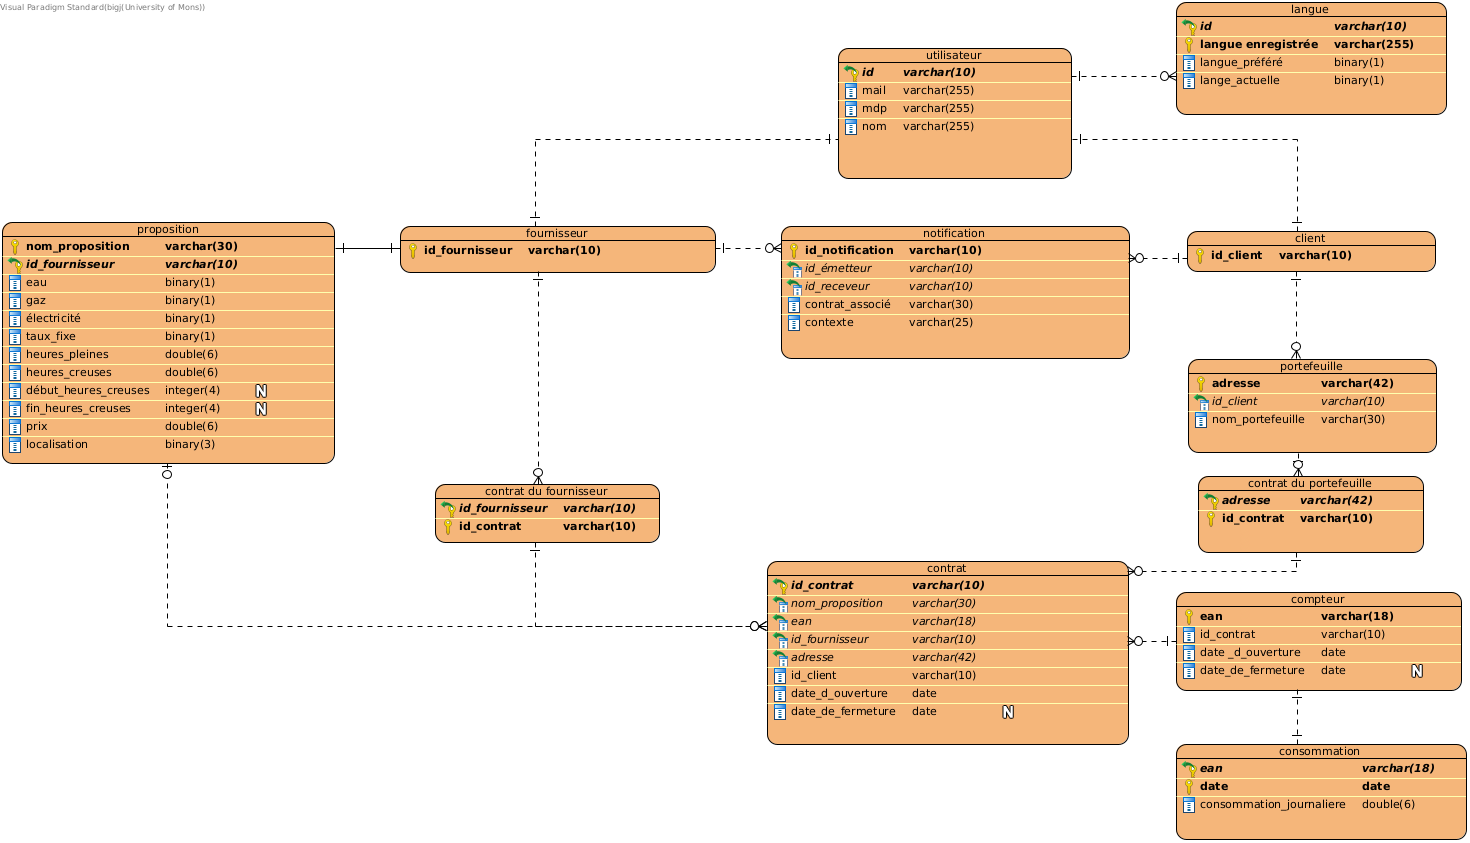
\includegraphics[scale=0.4]{bdd/bdd.png}
\end{figure}